%
% lie-gruppen.tex -- Lie-Gruppebn
%
% (c) 2020 Prof Dr Andreas Müller, Hochschule Rapperswil
%
\section{Lie-Gruppen
\label{buch:section:lie-gruppen}}
\rhead{Lie-Gruppen}
Die in bisherigen Beispielen untersuchten Matrizengruppen zeichnen sich
durch zusätzliche Eigenschaften aus.
Die Gruppe
\[
\operatorname{GL}_n(\mathbb{R}) 
=
\{ A \in M_n(\mathbb{R})\;|\; \det A \ne 0\}
\]
besteht aus den Matrizen, deren Determinante nicht $0$ ist.
Da die Menge der Matrizen mit $\det A=0$ eine abgeschlossene Menge
in $M_n(\mathbb{R}) \simeq \mathbb{R}^{n^2}$ ist, ist
$\operatorname{GL}_n(\mathbb{R})$ eine offene Teilmenge in $\mathbb{R}^{n^2}$,
sie besitzt also automatisch die Struktur einer $n^2$-Mannigfaltigkeit.
Dies gilt jedoch auch für alle anderen Matrizengruppen, die in diesem
Abschnitt genauer untersucht werden sollen.

\subsection{Mannigfaltigkeitsstruktur der Matrizengruppen
\label{buch:subsection:mannigfaltigkeitsstruktur-der-matrizengruppen}}
Eine Matrizengruppe wird automatsich zu einer Mannigfaltigkeit,
wenn es gelingt, eine Karte für eine Umgebung des neutralen Elements
zu finden.
Dazu muss gezeigt werden, dass sich aus einer solchen Karte für jedes
andere Gruppenelement eine Karte für eine Umgebung ableiten lässt.
Sei also $\varphi_e\colon U_e \to \mathbb{R}^N$ eine Karte für die Umgebung
$U_e\subset G$ von $e\in G$.
Für $g\in G$ ist dann die Abbildung
\[
\varphi_g
\colon
U_g
=
gU_e
\to
\mathbb{R}
:
h\mapsto \varphi_e(g^{-1}h)
\]
eine Karte für die Umgebung $U_g$ des Gruppenelementes $g$.
schreibt man $l_{g}$ für  die Abbildung $h\mapsto gh$, dann
kann man die Kartenabbildung auch $\varphi_g = \varphi_e\circ l_{g^{-1}}$
schreiben.

\subsubsection{Kartenwechsel}
Die Kartenwechsel-Abbildungen für zwei Karten $\varphi_{g_1}$
und $\varphi_{g_2}$ ist die Abbildung
\[
\varphi_{g_1,g_2}
=
\varphi_{g_1}\circ \varphi_{g_2}^{-1}
=
\varphi_e\circ l_{g_1^{-1}} \circ (\varphi_e\circ l_{g_2^{-1}})^{-1}
=
\varphi_e\circ l_{g_1^{-1}} \circ l_{g_2^{-1}}^{-1} \varphi_e^{-1}
=
\varphi_e\circ l_{g_1^{-1}} \circ l_{g_2}\varphi_e^{-1}
=
\varphi_e\circ l_{g_1^{-1}g_2}\varphi_e^{-1}
\]
mit der Ableitung
\[
D\varphi_e\circ Dl_{g_1^{-1}g_2} D\varphi_e^{-1}
=
D\varphi_e\circ Dl_{g_1^{-1}g_2} (D\varphi_e)^{-1}.
\]
Die Abbildung $l_{g_1^{-1}g_2}$ ist aber nur die Multiplikation mit
einer Matrix, also eine lineare Abbildung, so dass der Kartenwechsel
nichts anderes ist als die Darstellung der Matrix der Linksmultiplikation
$l_{g_1^{-1}g_2}$ im Koordinatensystem der Karte $U_e$ ist.
Differenzierbarkeit der Kartenwechsel ist damit sichergestellt,
die Matrizengruppen sind automatisch differenzierbare Mannigfaltigkeiten.

Die Konstruktion aller Karten aus einer einzigen Karte für eine
Umgebung des neutralen Elements zeigt auch, dass es für die Matrizengruppen
reicht, wenn man die Elemente in einer Umgebung des neutralen
Elementes parametrisieren kann.
Dies ist jedoch nicht nur für die Matrizengruppen möglich.
Wenn eine Gruppe gleichzeitig eine differenzierbare Mannigfaltigkeit
ist, dann können Karten über die ganze Gruppe transportiert werden,
wenn die Multiplikation mit Gruppenelementen eine differenzierbare
Abbildung ist.
Solche Gruppen heissen auch Lie-Gruppen gemäss der folgenden Definition.

\begin{definition}
\index{Lie-Gruppe}%
Eine {\em Lie-Gruppe} ist eine Gruppe, die gleichzeitig eine differenzierbare
Mannigfaltigkeit ist derart, dass die Abbildungen
\begin{align*}
G\times G \to G &: (g_1,g_2)\mapsto g_1g_2
\\
G\to G &: g \mapsto g^{-1}
\end{align*}
differenzierbare Abbildungen zwischen Mannigfaltigkeiten sind.
\end{definition}

Die Abstraktheit dieser Definition täuscht etwas über die 
Tatsache hinweg, dass sich mit Hilfe der Darstellungstheorie
jede beliebige Lie-Gruppe als Untermannigfaltigkeit einer 
Matrizengruppe verstehen lässt.
Das Studium der Matrizengruppen erlaubt uns daher ohne grosse
Einschränkungen ein Verständnis für die Theorie der Lie-Gruppen
zu entwickeln.

\subsubsection{Tangentialvektoren und die Exponentialabbildung}
Die Matrizengruppen sind alle in der
$n^2$-dimensionalen Mannigfaltigkeit $\operatorname{GL}_n(\mathbb{R})$
enthalten.
Diffferenzierbare Kurven $\gamma(t)$ in $\operatorname{GL}_n(\mathbb{R})$
haben daher in jedem Punkt Tangentialvektoren, die als Matrizen in
$M_n(\mathbb{R})$ betrachtet werden können.
Wenn $\gamma(t)$ die Matrixelemente $\gamma_{ij}(t)$ hat, dann ist der
Tangentialvektor im Punkt $\gamma(t)$ durch
\[
\frac{d}{dt}
\gamma(t)
=
\begin{pmatrix}
\dot{\gamma}_{11}(t)&\dots &\dot{\gamma}_{1n}(t)\\
\vdots              &\ddots&\vdots              \\
\dot{\gamma}_{n1}(t)&\dots &\dot{\gamma}_{nn}(t)
\end{pmatrix}
\]
gegeben.

Im Allgemeinen kann man Tangentialvektoren in verschiedenen Punkten
einer Mannigfaltigkeit nicht miteinander vergleichen.
Die Multiplikation $l_g$, die den Punkt $e$ in den Punkt $g$ verschiebt,
transportiert auch die Tangentialvektoren im Punkt $e$ in 
Tangentialvektoren im Punkt $g$.

\begin{aufgabe}
Gibt es eine Kurve $\gamma(t)\in\mathbb{GL}_n(\mathbb{R})$ mit
$\gamma(0)=e$ derart, dass der Tangentialvektor im Punkt $\gamma(t)$
für $t>0$ derselbe ist wie der Tangentialvektor im Punkt $e$, transportiert
durch Matrixmultiplikation mit $\gamma(t)$?
\end{aufgabe}

Eine solche Kurve muss die Differentialgleichung
\begin{equation}
\frac{d}{dt}\gamma(t)
=
\gamma(t)\cdot A
\label{buch:gruppen:eqn:expdgl}
\end{equation}
erfüllen, wobei $A\in M_n(\mathbb{R})$ der gegebene Tangentialvektor
in $e=I$ ist.

Die Matrixexponentialfunktion
\[
e^{At}
=
1+At+\frac{A^2t^2}{2!}+\frac{A^3t^3}{3!}+\frac{A^4t^4}{4!}+\dots
\]
liefert eine Einparametergruppe
$\mathbb{R}\to \operatorname{GL}_n(\mathbb{R})$ mit der Ableitung
\[
\frac{d}{dt} e^{At}
=
\lim_{h\to 0} \frac{e^{A(t+h)}-e^{At}}{h}
=
\lim_{h\to 0} e^{At}\frac{e^{Ah}-I}{h}
=
e^{At} A.
\]
Sie ist also Lösung der Differentialgleichung~\eqref{buch:gruppen:eqn:expdgl}.

\subsection{Drehungen in der Ebene
\label{buch:gruppen:drehungen2d}}
Die Drehungen der Ebene sind die orientierungserhaltenden Symmetrien
des Einheitskreises, der in Abbildung~\ref{buch:gruppen:fig:kartenkreis}
als Mannigfaltigkeit erkannt wurde.
Sie bilden eine Lie-Gruppe, die auf verschiedene Arten als Matrix
beschrieben werden kann.

\subsubsection{Die Untergruppe
$\operatorname{SO}(2)\subset \operatorname{GL}_2(\mathbb{R})$}
Drehungen der Ebene können in einer orthonormierten Basis durch
Matrizen der Form
\[
D_{\alpha}
=
\begin{pmatrix}
\cos\alpha&-\sin\alpha\\
\sin\alpha& \cos\alpha
\end{pmatrix}
\]
dargestellt werden.
Wir bezeichnen die Menge der Drehmatrizen in der Ebene mit
$\operatorname{SO}(2)\subset\operatorname{GL}_2(\mathbb{R})$.
Die Abbildung
\[
D_{\bullet}
\colon
\mathbb{R}\to \operatorname{SO}(2)
:
\alpha \mapsto D_{\alpha}
\]
hat die Eigenschaften
\begin{align*}
D_{\alpha+\beta}&= D_{\alpha}D_{\beta}
\\
D_0&=I
\\
D_{2k\pi}&=I\qquad \forall k\in\mathbb{Z}.
\end{align*}
Daraus folgt zum Beispiel, dass $D_{\bullet}$ eine $2\pi$-periodische
Funktion ist.
$D_{\bullet}$ bildet die Menge der Winkel $[0,2\pi)$ bijektiv auf
die Menge der Drehmatrizen in der Ebene ab.

Für jedes Intervall $(a,b)\subset\mathbb{R}$ mit Länge
$b-a < 2\pi$ ist die Abbildung $\alpha\mapsto D_{\alpha}$ umkehrbar,
die Umkehrung kann als Karte verwendet werden.
Zwei verschiedene Karten $\alpha_1\colon U_1\to\mathbb{R}$ und
$\alpha_2\colon U_2\to\mathbb{R}$ bilden die Elemente $g\in U_1\cap U_2$
in Winkel $\alpha_1(g)$ und $\alpha_2(g)$ ab, für die 
$D_{\alpha_1(g)}=D_{\alpha_2(g)}$ gilt.
Dies ist gleichbedeutend damit, dass $\alpha_1(g)=\alpha_2(g)+2\pi k$
mit $k\in \mathbb{Z}$.
In einem Intervall in $U_1\cap U_2$ muss $k$ konstant sein.
Die Kartenwechselabblidung ist also nur die Addition eines Vielfachen
von $2\pi$, mit der identischen Abbildung als Ableitung.
Diese Karten führen also auf besonders einfache Kartenwechselabbildungen.

\subsubsection{Die Untergruppe $S^1\subset\mathbb{C}$}
Ein alternatives Bild für die Drehungen der Ebene kann man in der komplexen
Ebene $\mathbb{C}$ erhalten.
Die Multiplikation mit der komplexen Zahl $e^{i\alpha}$ beschreibt eine
Drehung der komplexen Ebene um den Winkel $\alpha$.
Die Zahlen der Form $e^{i\alpha}$ haben den Betrag $1$ und die Abbildung
\[
f\colon \mathbb{R}\to \mathbb{C}:\alpha \mapsto e^{i\alpha}
\]
hat die Eigenschaften
\begin{align*}
f(\alpha+\beta) &= f(\alpha)f(\beta)
\\
f(0)&=1
\\
f(2\pi k)&=1\qquad\forall k\in\mathbb{Z},
\end{align*}
die zu den Eigenschaften der Abbildung $\alpha\mapsto D_{\alpha}$ 
analog sind.

Jede komplexe Zahl $z$ vom Betrag $1$ kann geschrieben werden in der Form
$z=e^{i\alpha}$, die Abbildung $f$ ist also eine Parametrisierung des
Einheitskreises in der Ebene.
Wir bezeichen $S^1=\{z\in\mathbb{C}\;|\; |z|=1\}$ die komplexen Zahlen vom
Betrag $1$.
$S^1$ ist eine Gruppe bezüglich der Multiplikation, da für jede Zahl
$z,w\in S^1$ gilt
$|z^{-1}|=1$ und $|zw|=1$ und damit $z^{-1}\in S^1$ und $zw\in S^1$.

Zu einer komplexen Zahl $z\in S^1$ gibt es einen bis auf Vielfache
von $2\pi$ eindeutigen Winkel $\alpha(z)$ derart, dass $e^{i\alpha(z)}=z$.
Damit kann man jetzt die Abbildung
\[
\varphi
\colon
S^1\to \operatorname{SO}(2)
:
z\mapsto  D_{\alpha(z)}
\]
konstruieren.
Da $D_{\alpha}$ $2\pi$-periodisch ist, geben um Vielfache
von $2\pi$ verschiedene Wahlen von $\alpha(z)$ die gleiche
Matrix $D_{\alpha(z)}$, die Abbildung $\varphi$ ist daher
wohldefiniert.
$\varphi$ erfüllt ausserdem die Bedingungen
\begin{align*}
\varphi(z_1z_2)
&=
D_{\alpha(z_1z_2)}
=
D_{\alpha(z_1)+\alpha(z_2)}
=
D_{\alpha(z_1)}D_{\alpha(z_2)}
=
\varphi(z_1)\varphi(z_2)
\\
\varphi(1)
&=
D_{\alpha(1)}
=
D_0
=
I
\end{align*}
Die Abbildung $\varphi$ ist ein Homomorphismus der Gruppe $S^1$
in die Gruppe $\operatorname{SO}(2)$.
Die Menge der Drehmatrizen in der Ebene kann also mit dem Einheitskreis
in der komplexen Ebene identifiziert werden.

\subsubsection{Tangentialvektoren von $\operatorname{SO}(2)$}
Da die Gruppe $\operatorname{SO}(2)$ eine eindimensionale Gruppe
ist, kann jede Kurve $\gamma(t)$ durch den Drehwinkel $\alpha(t)$
mit $\gamma(t) = D_{\alpha(t)}$ beschrieben werden.
Die Ableitung in $M_2(\mathbb{R})$ ist
\begin{align*}
\frac{d}{dt} \gamma(t)
&=
\frac{d}{d\alpha}
\begin{pmatrix}
\cos\alpha(t) & - \sin\alpha(t)\\
\sin\alpha(t) &   \cos\alpha(t)
\end{pmatrix}
\cdot
\frac{d\alpha}{dt}
\\
&=
\begin{pmatrix}
-\sin\alpha(t)&-\cos\alpha(t)\\
 \cos\alpha(t)&-\sin\alpha(t)
\end{pmatrix}
\cdot
\dot{\alpha}(t)
\\
&=
\begin{pmatrix}
\cos\alpha(t) & - \sin\alpha(t)\\
\sin\alpha(t) &   \cos\alpha(t)
\end{pmatrix}
\begin{pmatrix}
0&-1\\
1&0
\end{pmatrix}
\cdot
\dot{\alpha}(t)
=
D_{\alpha(t)}J\cdot\dot{\alpha}(t).
\end{align*}
Alle Tangentialvektoren von $\operatorname{SO}(2)$ im Punkt $D_\alpha$
entstehen aus $J$ durch Drehung mit der Matrix $D_\alpha$ und Skalierung
mit $\dot{\alpha}(t)$.

%
% Isometrien von R^n
%
\subsection{Isometrien von $\mathbb{R}^n$
\label{buch:gruppen:isometrien}}

\subsubsection{Skalarprodukt}
Lineare Abbildungen des Raumes $\mathbb{R}^n$ können durch
$n\times n$-Matrizen beschrieben werden.
Die Matrizen, die das Standardskalarprodukt $\mathbb{R}^n$ erhalten,
bilden eine Gruppe, die in diesem Abschnitt genauer untersucht werden soll.
Eine Matrix $A\in M_{n}(\mathbb{R})$ ändert das Skalarprodukt, wenn
für jedes beliebige Paar $x,y$ von Vektoren gilt
$\langle Ax,Ay\rangle = \langle x,y\rangle$.
Das Standardskalarprodukt kann mit dem Matrixprodukt ausgedrückt werden:
\[
\langle Ax,Ay\rangle
=
(Ax)^tAy
=
x^tA^tAy
=
x^ty
=
\langle x,y\rangle
\]
für jedes Paar von Vektoren $x,y\in\mathbb{R}$.

Mit dem Skalarprodukt kann man auch die Matrixelemente einer Matrix
einer Abbildung $f$ in der Standardbasis bestimmen.
Das Skalarprodukt $\langle e_i, v\rangle$ ist die Länge der Projektion
des Vektors $v$ auf die Richtung $e_i$.
Die Komponenten von $Ae_j$ sind daher $a_{ij}=\langle e_i,f(e_j)\rangle$.
Die Matrix $A$ der Abbildung $f$ hat also die Matrixelemente
$a_{ij}=e_i^tAe_j$.

\subsubsection{Die orthogonale Gruppe $\operatorname{O}(n)$}
Die Matrixelemente von $A^tA$ sind
$\langle A^tAe_i, e_j\rangle =\langle e_i,e_j\rangle = \delta_{ij}$
sind diejenigen der Einheitsmatrix,
die Matrix $A$ erfüllt $AA^t=I$ oder $A^{-1}=A^t$.
Dies sind die {\em orthogonalen} Matrizen.
Die Menge $\operatorname{O}(n)$ der isometrischen Abbildungen besteht
daher aus den Matrizen
\[
\operatorname{O}(n)
=
\{ A\in M_n(\mathbb{R})\;|\; AA^t=I\}.
\]
Die Matrixgleichung $AA^t=I$ liefert $n(n+1)/2$ unabhängige Bedingungen,
die die orthogonalen Matrizen innerhalb der $n^2$-dimensionalen
Menge $M_n(\mathbb{R})$ auszeichnen.
Die Menge $\operatorname{O}(n)$ der orthogonalen Matrizen hat daher
die Dimension
\[
n^2 - \frac{n(n+1)}{2}
=
\frac{2n^2-n^2-n}{2}
=
\frac{n(n-1)}2.
\]
Im Spezialfall $n=2$ ist die Gruppe $O(2)$ eindimensional.

\subsubsection{Tangentialvektoren}
Die orthogonalen Matrizen bilden eine abgeschlossene Untermannigfaltigkeit
von $\operatorname{GL}_n(\mathbb{R})$, nicht jede Matrix $M_n(\mathbb{R})$ 
kann also ein Tangentialvektor von $O(n)$ sein.
Um herauszufinden, welche Matrizen als Tangentialvektoren in Frage
kommen, betrachten wir eine Kurve $\gamma\colon\mathbb{R}\to O(n)$
von orthogonalen Matrizen mit $\gamma(0)=I$.
Orthogonal bedeutet 
\[
\begin{aligned}
&&
0
&=
\frac{d}{dt}I
=
\frac{d}{dt}
(\gamma(t)^t\gamma(t))
=
\dot{\gamma}(t)^t\gamma(t))
+
\gamma(t)^t\dot{\gamma}(t))
\\
&\Rightarrow&
0
&=
\dot{\gamma}(0)^t \cdot I + I\cdot \dot{\gamma(0)}
=
\dot{\gamma}(0)^t + \dot{\gamma}(0)
=
A^t+A=0
\\
&\Rightarrow&
A^t&=-A
\end{aligned}
\]
Die Tangentialvektoren von $\operatorname{O}(n)$ sind also genau
die antisymmetrischen Matrizen.

Für $n=2$ sind alle antisymmetrischen Matrizen Vielfache der Matrix
$J$, wie in Abschnitt~\ref{buch:gruppen:drehungen2d}
gezeigt wurde.

Für jedes Paar $i<j$ ist die Matrix $A_{ij}$ mit den Matrixelementen
$(A_{ij})_{ij}=-1$ und $(A_{ij})_{ji}=1$
antisymmetrisch.
Für $n=2$ ist $A_{12}=J$.
Die $n(n-1)/2$ Matrizen $A_{ij}$ bilden eine Basis des
$n(n-1)/2$-dimensionale Tangentialraumes von $\operatorname{O}(n)$.

Tangentialvektoren in einem anderen Punkt $g\in\operatorname{O}(n)$
haben die Form $gA$, wobei $A$ eine antisymmetrische Matrix ist.
Diese Matrizen sind nur noch in speziellen Fällen antisymmetrisch,
zum Beispiel im Punkt $-I\in\operatorname{O}(n)$.

\subsubsection{Die Gruppe $\operatorname{SO}(n)$}
Die Gruppe $\operatorname{O}(n)$ enhält auch Isometrien, die
die Orientierung des Raumes umkehren, wie zum Beispiel Spiegelungen.
Wegen $\det (AA^t)=\det A\det A^t = (\det A)^2=1$ kann die Determinante
einer orthogonalen Matrix nur $\pm 1$ sein.
Orientierungserhaltende Isometrien haben Determinante $1$.

Die Gruppe
\[
\operatorname{SO}(n)
=
\{A\in\operatorname{O}(n)\;|\; \det A=1\}
\]
heisst die {\em spezielle orthogonale Gruppe}.
Die Dimension der Gruppe $\operatorname{O}(n)$ ist $n(n-1)/2$.

\subsubsection{Die Gruppe $\operatorname{SO}(3)$}
Die Gruppe $\operatorname{SO}(3)$ der Drehungen des dreidimensionalen
Raumes hat die Dimension $3(3-1)/2=3$.
Eine Drehung wird festgelegt durch die Richtung der Drehachse und den
Drehwinkel.
Die Richtung der Drehachse ist ein Einheitsvektor, also ein Punkt
auf der zweidimensionalen Kugel.
Der Drehwinkel ist der dritte Parameter.

Drehungen mit kleinen Drehwinkeln können zusammengesetzt werden
aus den Matrizen
\begin{align*}
D_{x,\alpha}
&=
\begin{pmatrix}
1&0&0\\
0&\cos\alpha&-\sin\alpha\\
0&\sin\alpha& \cos\alpha
\end{pmatrix},
&
D_{y,\beta}
&=
\begin{pmatrix}
 \cos\beta&0&\sin\beta\\
      0    &1&     0    \\
-\sin\beta&0&\cos\beta
\end{pmatrix},
&
D_{z,\gamma}
&=
\begin{pmatrix}
\cos\gamma&-\sin\gamma&0\\
\sin\gamma& \cos\gamma&0\\
    0     &     0     &1
\end{pmatrix}
\\
&=
e^{A_{23}t}
&
&=
e^{-A_{13}t}
&
&=
e^{A_{21}t}
\end{align*}
die Drehungen um die Koordinatenachsen um den Winkel $\alpha$
beschreiben.
Auch die Winkel $\alpha$, $\beta$ und $\gamma$ können als die
drei Koordinaten der Mannigkfaltigkeit $\operatorname{SO}(3)$
angesehen werden.

%
% Spezielle lineare Gruppe
%
\subsection{Volumenerhaltende Abbildungen und
die Gruppe $\operatorname{SL}_n(\mathbb{R})$
\label{buch:gruppen:sl}}
Die Elemente der Gruppe $SO(n)$ erhalten Längen, Winkel und die
Orientierung, also auch das Volumen.
Es gibt aber volumenerhaltende Abbildungen, die Längen oder Winkel
nicht notwendigerweise erhalten.
Matrizen $A\in M_n(\mathbb{R})$, die das Volumen erhalten,
haben die Determinante $\det A=1$.
Wegen $\det(AB)=\det A\det B$ ist das Produkt zweier Matrizen mit
Determinante $1$ wieder eine solche, sie bilden daher eine Gruppe.

\begin{definition}
Die volumenerhaltenden Abbildungen bilden die Gruppe
\[
\operatorname{SL}_n(\mathbb{R})
=
\{
A\in M_n(\mathbb{R})
\;|\;
\det (A) = 1
\}
\]
sie heisst die {\em spezielle lineare Gruppe}.
\end{definition}

Wir wollen jetzt die Tangentialvektoren von $\operatorname{SL}_n(\mathbb{R})$
bestimmen.
Dazu sei $A(t)$ eine Kurve in $\operatorname{SL}_n(\mathbb{R})$
mit $A(0)=I$.
Für alle $t\in\mathbb{R}$ ist $\det A(t)=1$, daher ist die Ableitung
\[
\frac{d}{dt} \det A(t) = 0
\quad\text{an der Stelle $t=0$.}
\]
Für $n=2$ ist
\begin{align*}
A(t)
&=
\begin{pmatrix}
a(t)&b(t)\\
c(t)&d(t)
\end{pmatrix}
\in
\operatorname{SL}_2(\mathbb{R})
&&\Rightarrow&
\frac{d}{dt}
\det A(t)\bigg|_{t=0}
&=
\dot{a}(0) d(0)+a(0)\dot{d}(0)
-
\dot{b}(0) c(0)-b(0)\dot{c}(0)
\\
&&&&
&=
\dot{a}(0) + \dot{d}(0)
\\
&&&&
&=
\operatorname{Spur}\frac{dA}{dt}.
\end{align*}
Dies gilt nicht nur im Falle $n=2$, sondern ganz allgemein für beliebige
$n\times n$-Matrizen.

\begin{satz}
Ist $A(t)$ eine differenzierbare Kurve in $\operatorname{SL}_n(\mathbb{B})$
mit $A(0)=I$, dann ist $\operatorname{Spur}\dot{A}(0)=0$.
\end{satz}

\begin{proof}[Beweis]
Die Entwicklung der Determinante von $A$ nach der ersten Spalte ist
\[
\det A(t) = \sum_{i=1}^n (-1)^{i+1} a_{i1}(t) \det A_{i1}(t).
\]
Die Ableitung nach $t$ ist
\[
\frac{d}{dt} \det A(t)
=
\sum_{i=1}^n (-1)^{i+1} \dot{a}_{i1}(t) \det A_{i1}(t).
+
\sum_{i=1}^n (-1)^{i+1} a_{i1}(t) \frac{d}{dt}\det A_{i1}(t).
\]
An der Stelle $t=0$ enthält $\det A_{i1}(0)$ für $i\ne 1$
eine Nullzeile, der einzige nichtverschwindende Term in der ersten
Summe ist daher der erste.
In der zweiten Summe ist das einzige nicht verschwindende $a_{i1}(0)$
jenes für $i=1$, somit ist die Ableitung von $\det A(t)$
\begin{equation}
\frac{d}{dt} \det A(t)
=
\dot{a}_{11}(t) \det A_{11}(t).
+
\frac{d}{dt}\det A_{11}(t)
=
\dot{a}_{11}(0) 
+
\frac{d}{dt}\det A_{11}(t).
\label{buch:gruppen:eqn:detspur}
\end{equation}
Die Beziehung \eqref{buch:gruppen:eqn:detspur} kann für einen Beweis mit
vollständiger Induktion verwendet werden.

Die Induktionsverankerung für $n=1$ besagt, dass $\det A(t)=a_{11}(t)$
genau dann konstant $=1$ ist, wenn $\dot{a}_{11}(0)=\operatorname{Spur}A(0)$
ist.
Unter der Induktionsannahme, dass für eine $(n-1)\times(n-1)$-Matrix
$\tilde{A}(t)$ mit $\tilde{A}(0)=I$ die Ableitung der Determinante
\[
\frac{d}{dt}\tilde{A}(0)
=
\operatorname{Spur}\dot{\tilde{A}}(0)
\]
ist, folgt jetzt mit
\eqref{buch:gruppen:eqn:detspur}, dass
\[
\frac{d}{dt}A(0)
=
\dot{a}_{11}(0)
+
\frac{d}{dt} \det A_{11}(t)\bigg|_{t=0}
=
\dot{a}_{11}(0)
+
\operatorname{Spur}\dot{A}_{11}(0)
=
\operatorname{Spur}\dot{A}(0).
\]
Damit folgt jetzt die Behauptung für alle $n$.
\end{proof}

\begin{beispiel}
Die Tangentialvektoren von $\operatorname{SL}_2(\mathbb{R})$ sind 
die spurlosen Matrizen
\[
A=\begin{pmatrix}a&b\\c&d\end{pmatrix}
\quad\Rightarrow\quad
\operatorname{Spur}A=a+d=0
\quad\Rightarrow\quad
A=\begin{pmatrix}a&b\\c&-a\end{pmatrix}.
\]
Der Tangentialraum ist also dreidimensional.
Als Basis könnte man die folgenden Vektoren verwenden:
\begin{align*}
A
&=
\begin{pmatrix}1&0\\0&-1\end{pmatrix}
&&\Rightarrow&
e^{At}
&=
\begin{pmatrix} e^t & 0 \\ 0 & e^{-t} \end{pmatrix}
\\
B
&=
\begin{pmatrix}0&-1\\1&0\end{pmatrix}
&&\Rightarrow&
e^{Bt}
&=
\begin{pmatrix}
\cos t & -\sin t\\
\sin t &  \cos t
\end{pmatrix}
\\
C
&=
\begin{pmatrix}0&1\\1&0\end{pmatrix}
&&\Rightarrow&
e^{Ct}
&=
I + Ct + \frac{C^2t^2}{2!} + \frac{C^3t^3}{3!} + \frac{C^4t^4}{4!}+\dots
\\
&&&&
&=
I\biggl(1 + \frac{t^2}{2!} + \frac{t^4}{4!}+\dots \biggr)
+
C\biggl(t + \frac{t^3}{3!} + \frac{t^5}{5!}+\dots \biggr)
\\
&&&&
&=
I\cosh t + C \sinh t
=
\begin{pmatrix}
\cosh t & \sinh t\\
\sinh t & \cosh t
\end{pmatrix},
\end{align*}
wobei in der Auswertung der Potenzreihe für $e^{Ct}$ verwendet wurde,
dass $C^2=I$.

Die Matrizen $e^{At}$ Streckungen der einen Koordinatenachse und
Stauchungen der anderen derart, dass das Volumen erhalten bleibt.
Die Matrizen $e^{Bt}$ sind Drehmatrizen, die Längen und Winkel und
damit erst recht den Flächeninhalt erhalten.
Die Matrizen der Form $e^{Ct}$ haben die Vektoren $(1,\pm1)$ als
Eigenvektoren:
\begin{align*}
\begin{pmatrix}1\\1\end{pmatrix}
&\mapsto
e^{Ct}
\begin{pmatrix}1\\1\end{pmatrix}
=
(\cosh t +\sinh t)
\begin{pmatrix}1\\1\end{pmatrix}
=
\biggl(
\frac{e^t+e^{-t}}2
+
\frac{e^t-e^{-t}}2
\biggr)
\begin{pmatrix}1\\1\end{pmatrix}
=
e^t
\begin{pmatrix}1\\1\end{pmatrix}
\\
\begin{pmatrix}1\\-1\end{pmatrix}
&\mapsto
e^{Ct}
\begin{pmatrix}1\\-1\end{pmatrix}
=
(\cosh t -\sinh t)
\begin{pmatrix}1\\-1\end{pmatrix}
=
\biggl(
\frac{e^t+e^{-t}}2
-
\frac{e^t-e^{-t}}2
\biggr)
\begin{pmatrix}1\\-1\end{pmatrix}
=
e^{-t}
\begin{pmatrix}1\\-1\end{pmatrix}
\end{align*}
Die Matrizen $e^{Ct}$ strecken die Richtung $(1,1)$ um $e^t$ und
die dazu orthogonale Richtung $(1,-1)$ um den Faktor $e^{-t}$.
Dies ist die gegenüber $e^{At}$ um $45^\circ$ verdrehte Situation,
auch diese Matrizen sind flächenerhaltend.
\begin{figure}
\centering
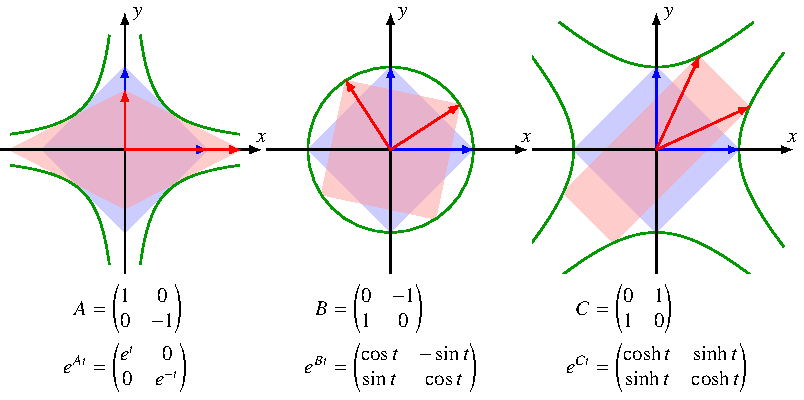
\includegraphics{chapters/60-gruppen/images/sl2.pdf}
\caption{Tangentialvektoren und die davon erzeugen Einparameteruntergruppen
für die Lie-Gruppe $\operatorname{SL}_2(\mathbb{R})$ der flächenerhaltenden
linearen Abbildungen von $\mathbb{R}^2$.
In allen drei Fällen wird ein blauer Rhombus mit den Ecken in den
Standardbasisvektoren von einer Matrix der Einparameteruntergruppe zu
zum roten Viereck verzerrt, der Flächeninhalt bleibt aber erhalten.
In den beiden Fällen $B$ und $C$ stellen die grünen Kurven die Bahnen
der Bilder der Standardbasisvektoren dar.
\label{buch:gruppen:fig:sl2}}
\end{figure}%
\begin{figure}
\centering
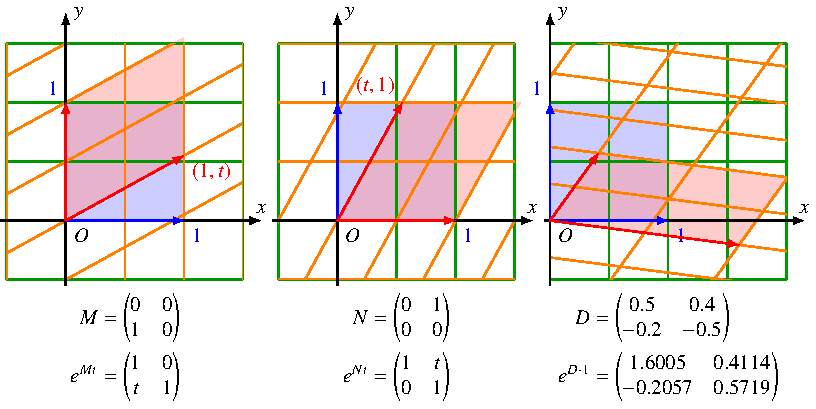
\includegraphics{chapters/60-gruppen/images/scherungen.pdf}
\caption{Weitere Matrizen mit Spur $0$ und ihre Wirkung 
Die inken beiden Beispiele $M$ und $N$ sind nilpotente Matrizen,
die zugehörigen Einparameter-Untergruppen beschreiben Schwerungen.
\label{buch:gruppen:fig:scherungen}}
\end{figure}
\end{beispiel}

%
% Die Gruppe SU(2)
%
\subsection{Die Gruppe $\operatorname{SU}(2)$
\label{buch:gruppen:su2}}
Die Menge der Matrizen
\[
\operatorname{SU}(2)
=
\left\{
\left.
A=\begin{pmatrix} a&b\\c&d\end{pmatrix}
\;\right|\;
a,b,c,d\in\mathbb{C},\det(A)=1, AA^*=I
\right\}
\]
heisst die {\em spezielle unitäre Gruppe}.
Wegen $\det(AB)=\det(A)\det(B)=1$ und $(AB)^*AB=B^*A^*AB=B^*B=I$ ist 
$\operatorname{SU}(2)$ eine Untergruppe von $\operatorname{GL}_2(\mathbb{C})$.
Die Bedingungen $\det A=1$ und $AA^*=I$ schränken die möglichen Werte
von $a$ und $b$ weiter ein.
Aus 
\[
A^*
=
\begin{pmatrix}
\overline{a}&\overline{c}\\
\overline{b}&\overline{d}
\end{pmatrix}
\]
und den Bedingungen führen die Gleichungen
\[
\begin{aligned}
a\overline{a}+b\overline{b}&=1
&&\Rightarrow&|a|^2+|b|^2&=1
\\
a\overline{c}+b\overline{d}&=0
&&\Rightarrow&
\frac{a}{b}&=-\frac{\overline{d}}{\overline{c}}
\\
c\overline{a}+d\overline{b}&=0
&&\Rightarrow&
\frac{c}{d}&=-\frac{\overline{b}}{\overline{a}}
\\
c\overline{c}+d\overline{d}&=1&&\Rightarrow&|c|^2+|d|^2&=1
\\
ad-bc&=1
\end{aligned}
\]
Aus der zweiten Gleichung kann man ableiten, dass es eine Zahl $t\in\mathbb{C}$
gibt derart, dass $c=-t\overline{b}$ und $d=t\overline{a}$.
Damit wird die Bedingung an die Determinante zu
\[
1
=
ad-bc = at\overline{a} - b(-t\overline{b})
=
t(|a|^2+|b|^2)
=
t,
\]
also muss die Matrix $A$ die Form haben
\[
A
=
\begin{pmatrix}
a&b\\
-\overline{b}&\overline{a}
\end{pmatrix}
\qquad\text{mit}\quad |a|^2+|b|^2=1.
\]
Schreibt man $a=a_1+ia_2$ und $b=b_1+ib_2$ mit rellen $a_i$ und $b_i$,
dann besteht $SU(2)$  aus den Matrizen der Form
\[
A=
\begin{pmatrix}
 a_1+ia_2&b_1+ib_2\\
-b_1+ib_2&a_1-ia_2
\end{pmatrix}
\]
mit der zusätzlichen Bedingung
\[
|a|^2+|b|^2
=
a_1^2 + a_2^2 + b_1^2 + b_2^2 = 1.
\]
Die Matrizen von $\operatorname{SU}(2)$ stehen daher in einer
eins-zu-eins-Beziehung zu den Vektoren $(a_1,a_2,b_1,b_2)\in\mathbb{R}^4$
eines vierdimensionalen reellen Vektorraums mit Länge $1$.
Geometrisch betrachtet ist also $\operatorname{SU}(2)$ eine dreidmensionalen
Kugel, die in einem vierdimensionalen Raum eingebettet ist.



